\documentclass[tikz,border=10pt]{standalone}
\usepackage{graphicx}
\usepackage{tikz}
\usetikzlibrary{positioning, fit, calc}

\begin{document}

\begin{tikzpicture}[
    x={3cm/1344}, % Scaling to match the 1344x768 image
    y={1.71cm/768},
    anchor=north west,
    font=\sffamily
]

    % Load ground truth image (Left)
    \node[inner sep=0, anchor=north west] (img) at (0,500)
      {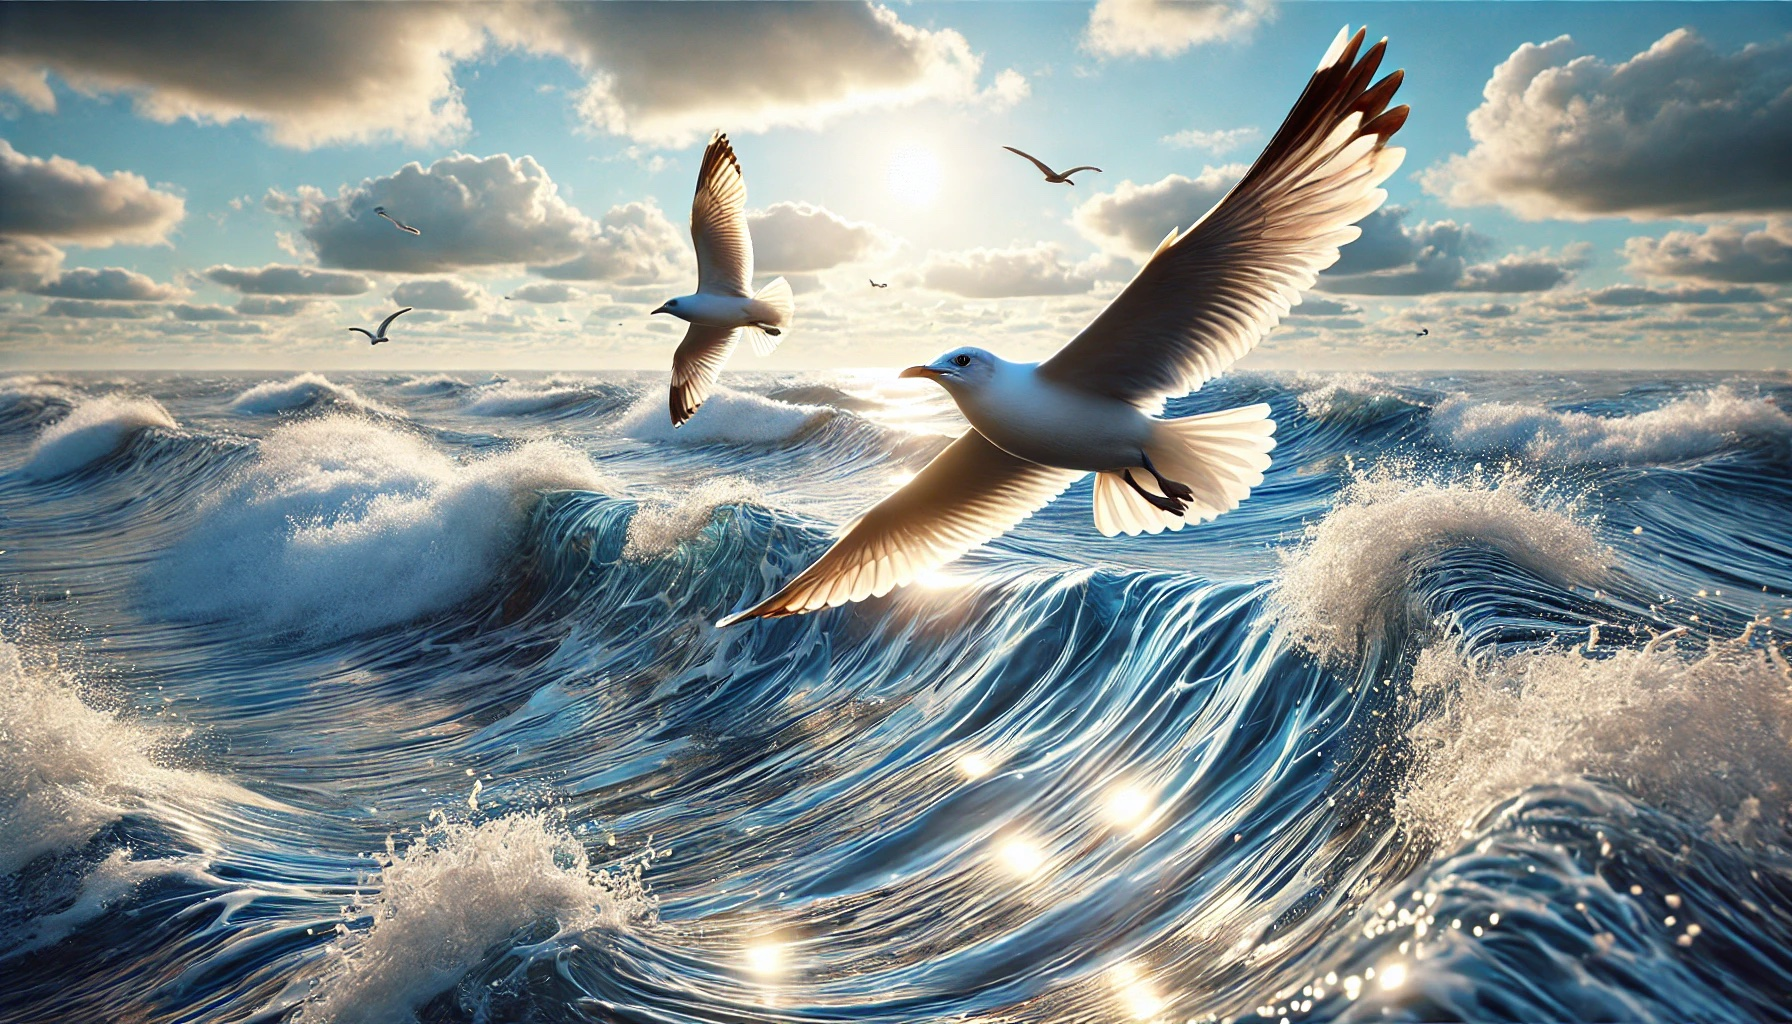
\includegraphics[width=3cm]{gulls.jpg}};

    % Define bounding box colors
    \definecolor{box1}{RGB}{255,0,0}   % Red (Left Gull)
    \definecolor{box2}{RGB}{0,0,255}   % Blue (Right Gull)

    % Ground Truth Bounding Boxes (Matching 1344x768)
    \coordinate (leftBox1NW) at (460,200);
    \coordinate (leftBox1SE) at (620,340);
    \coordinate (leftBox2NW) at (680,120);
    \coordinate (leftBox2SE) at (920,300);

    % Draw Ground Truth Bounding Boxes
    \draw[line width=2pt, color=box1] (leftBox1NW) rectangle (leftBox1SE);
    \draw[line width=2pt, color=box2] (leftBox2NW) rectangle (leftBox2SE);

    % Labels
    \node[above] at (670,550) {\textbf{Ground Truth Boxes}};
    \node[above] at (2514,518) {\textbf{Low-Noise Bounding Boxes}};
    \node[above] at (2514,518-1268) {\textbf{High-Noise Bounding Boxes}};

    % Offset for low/high noise versions
    \pgfmathsetmacro{\shiftX}{1844} % Image width in px
    \pgfmathsetmacro{\gap}{50}      % Extra gap between images

    % Low-Noise Bounding Boxes (Top Right)
    \node[inner sep=0, anchor=north west] (imgLow) at (\shiftX+\gap,500)
      {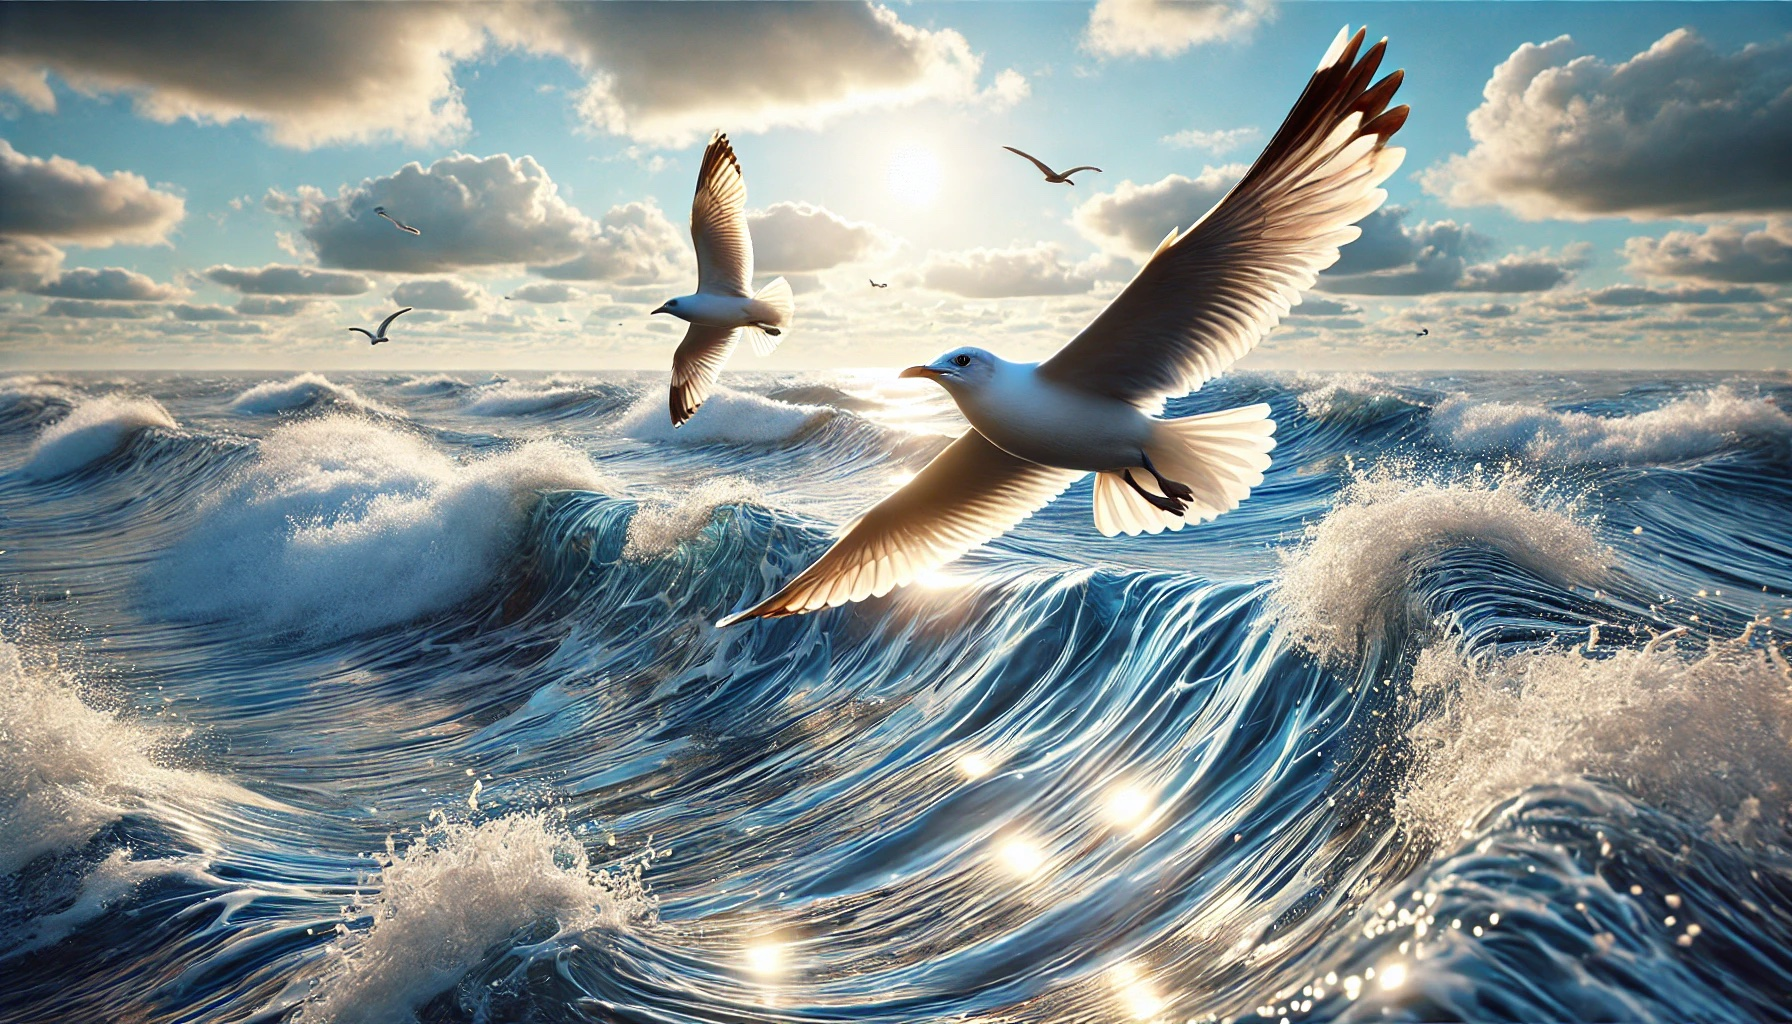
\includegraphics[width=3cm]{gulls.jpg}};

    \coordinate (lowNoise1NW) at (\shiftX+\gap+465, 205);
    \coordinate (lowNoise1SE) at (\shiftX+\gap+615, 335);
    \coordinate (lowNoise2NW) at (\shiftX+\gap+685, 125);
    \coordinate (lowNoise2SE) at (\shiftX+\gap+915, 295);

    \draw[line width=2pt, color=box1, dashed] (lowNoise1NW) rectangle (lowNoise1SE);
    \draw[line width=2pt, color=box2, dashed] (lowNoise2NW) rectangle (lowNoise2SE);

    % High-Noise Bounding Boxes (Bottom Right)
    \node[inner sep=0, anchor=north west] (imgHigh) at (\shiftX+\gap,-868)
      {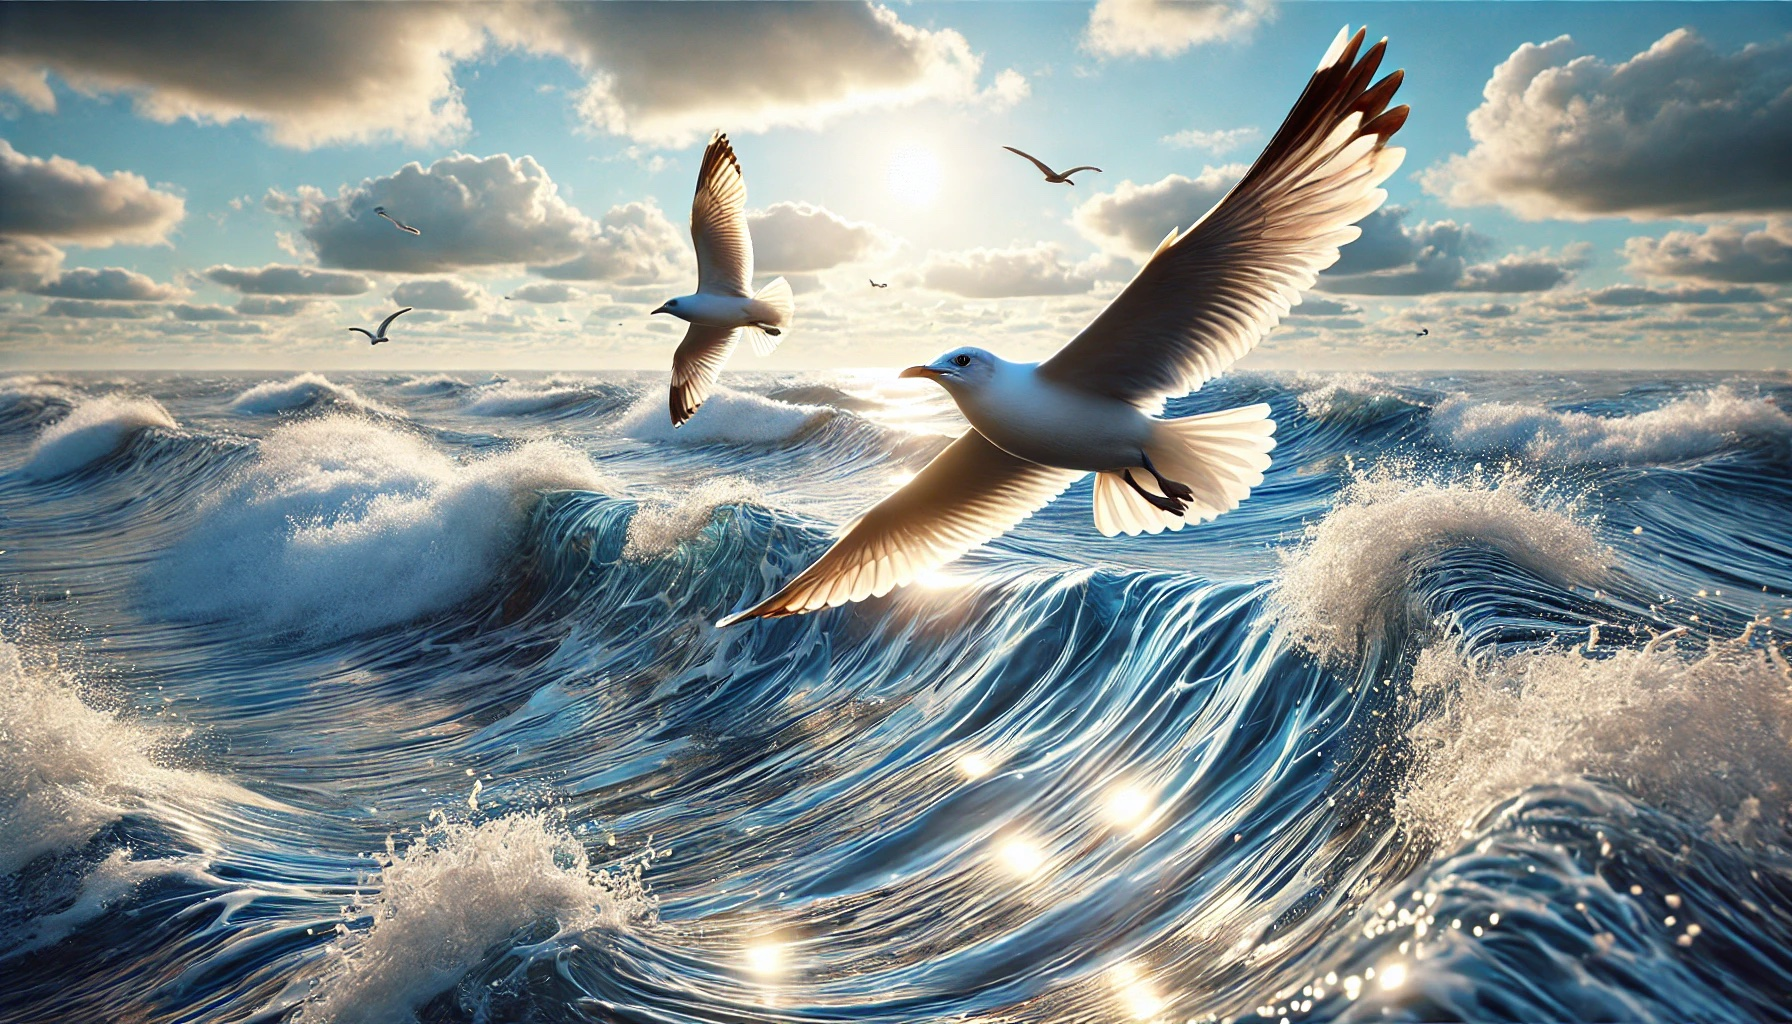
\includegraphics[width=3cm]{gulls.jpg}};

    \coordinate (highNoise1NW) at (\shiftX+\gap+250, 220-1268);
    \coordinate (highNoise1SE) at (\shiftX+\gap+430, 360-1268);
    \coordinate (highNoise2NW) at (\shiftX+\gap+870, 140-1268);
    \coordinate (highNoise2SE) at (\shiftX+\gap+1130, 320-1268);

    \draw[line width=2pt, color=box1, dashed] (highNoise1NW) rectangle (highNoise1SE);
    \draw[line width=2pt, color=box2, dashed] (highNoise2NW) rectangle (highNoise2SE);

    % Correspondence Arrows (Low Noise)
    \draw[->, thick, color=box1] ($(leftBox1NW)!0.5!(leftBox1SE)$) -- ($(lowNoise1NW)!0.5!(lowNoise1SE)$);
    \draw[->, thick, color=box2] ($(leftBox2NW)!0.5!(leftBox2SE)$) -- ($(lowNoise2NW)!0.5!(lowNoise2SE)$);

    % Correspondence Arrows (High Noise)
    \draw[->, thick, color=box1] ($(leftBox1NW)!0.5!(leftBox1SE)$) -- ($(highNoise1NW)!0.5!(highNoise1SE)$);
    \draw[->, thick, color=box2] ($(leftBox2NW)!0.5!(leftBox2SE)$) -- ($(highNoise2NW)!0.5!(highNoise2SE)$);

\end{tikzpicture}

\end{document}
